\documentclass{standalone}
\usepackage{tikz}
\usetikzlibrary{patterns, positioning}


\begin{document}
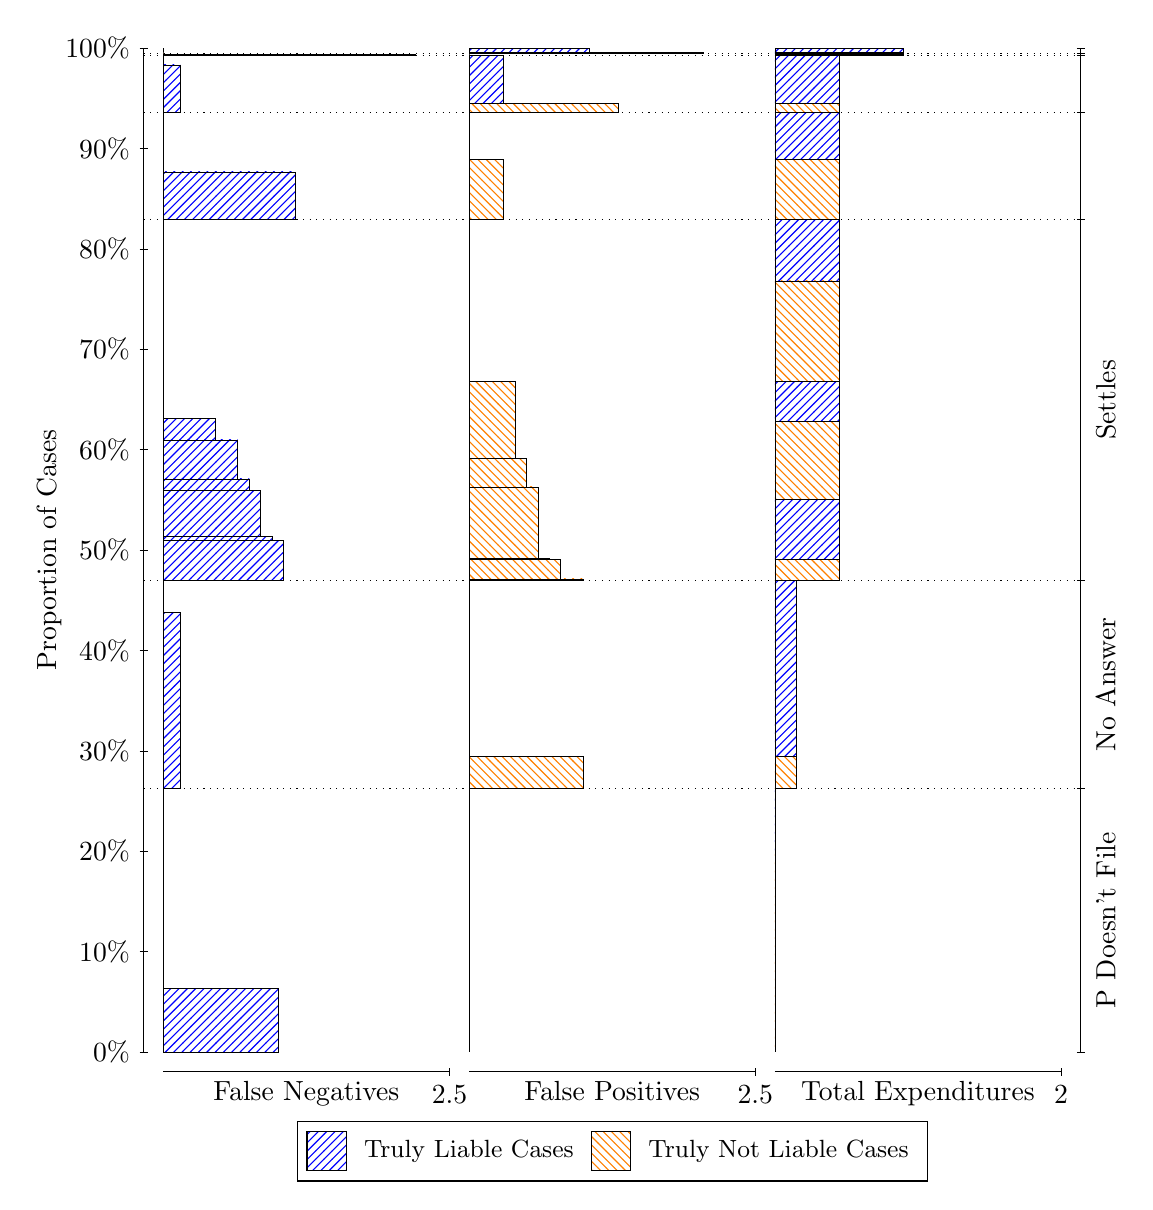
\begin{tikzpicture}
\draw[black, very thin] (1.5,1.75) -- (1.5,14.5);
\node[rotate=90, text=black, anchor=center] at (0.3, 8.125) {Proportion of Cases};
\draw[black, very thin] (1.45,1.75) -- (1.55,1.75);
\node[text=black, anchor=east] at (1.45, 1.75) {0\%};
\draw[black, very thin] (1.45,3.025) -- (1.55,3.025);
\node[text=black, anchor=east] at (1.45, 3.025) {10\%};
\draw[black, very thin] (1.45,4.3) -- (1.55,4.3);
\node[text=black, anchor=east] at (1.45, 4.3) {20\%};
\draw[black, very thin] (1.45,5.575) -- (1.55,5.575);
\node[text=black, anchor=east] at (1.45, 5.575) {30\%};
\draw[black, very thin] (1.45,6.85) -- (1.55,6.85);
\node[text=black, anchor=east] at (1.45, 6.85) {40\%};
\draw[black, very thin] (1.45,8.125) -- (1.55,8.125);
\node[text=black, anchor=east] at (1.45, 8.125) {50\%};
\draw[black, very thin] (1.45,9.4) -- (1.55,9.4);
\node[text=black, anchor=east] at (1.45, 9.4) {60\%};
\draw[black, very thin] (1.45,10.675) -- (1.55,10.675);
\node[text=black, anchor=east] at (1.45, 10.675) {70\%};
\draw[black, very thin] (1.45,11.95) -- (1.55,11.95);
\node[text=black, anchor=east] at (1.45, 11.95) {80\%};
\draw[black, very thin] (1.45,13.225) -- (1.55,13.225);
\node[text=black, anchor=east] at (1.45, 13.225) {90\%};
\draw[black, very thin] (1.45,14.5) -- (1.55,14.5);
\node[text=black, anchor=east] at (1.45, 14.5) {100\%};

\draw[black, very thin] (13.4,1.75) -- (13.4,14.5);
\draw[black, very thin] (13.35,1.75) -- (13.45,1.75);
\node[anchor=west] at (13.35, 1.75) {};
\draw[black, very thin] (13.35,5.0974) -- (13.45,5.0974);
\node[anchor=west] at (13.35, 5.0974) {};
\draw[black, very thin] (13.35,7.7383) -- (13.45,7.7383);
\node[anchor=west] at (13.35, 7.7383) {};
\draw[black, very thin] (13.35,12.325) -- (13.45,12.325);
\node[anchor=west] at (13.35, 12.325) {};
\draw[black, very thin] (13.35,13.683) -- (13.45,13.683);
\node[anchor=west] at (13.35, 13.683) {};
\draw[black, very thin] (13.35,14.402) -- (13.45,14.402);
\node[anchor=west] at (13.35, 14.402) {};
\draw[black, very thin] (13.35,14.43) -- (13.45,14.43);
\node[anchor=west] at (13.35, 14.43) {};
\draw[black, very thin] (13.35,14.5) -- (13.45,14.5);
\node[anchor=west] at (13.35, 14.5) {};

\draw[black, very thin, pattern color=blue, pattern=north east lines] (1.75,1.75) rectangle (3.2033,2.5562);
\draw[black, very thin, pattern color=orange, pattern=north west lines] (1.75,2.5562) rectangle (1.75,5.0974);
\draw[black, very thin, pattern color=blue, pattern=north east lines] (1.75,5.0974) rectangle (1.968,7.3347);
\draw[black, very thin, pattern color=orange, pattern=north west lines] (1.75,7.3347) rectangle (1.75,7.7383);
\draw[black, very thin, pattern color=blue, pattern=north east lines] (1.75,7.7383) rectangle (3.276,8.2478);
\draw[black, very thin, pattern color=blue, pattern=north east lines] (1.75,8.2478) rectangle (3.1307,8.2981);
\draw[black, very thin, pattern color=blue, pattern=north east lines] (1.75,8.2981) rectangle (2.9853,8.8839);
\draw[black, very thin, pattern color=blue, pattern=north east lines] (1.75,8.8839) rectangle (2.84,9.0283);
\draw[black, very thin, pattern color=blue, pattern=north east lines] (1.75,9.0283) rectangle (2.6947,9.5242);
\draw[black, very thin, pattern color=blue, pattern=north east lines] (1.75,9.5242) rectangle (2.404,9.7958);
\draw[black, very thin, pattern color=orange, pattern=north west lines] (1.75,9.7958) rectangle (1.75,12.325);
\draw[black, very thin, pattern color=blue, pattern=north east lines] (1.75,12.325) rectangle (3.4213,12.926);
\draw[black, very thin, pattern color=orange, pattern=north west lines] (1.75,12.926) rectangle (1.75,13.683);
\draw[black, very thin, pattern color=blue, pattern=north east lines] (1.75,13.683) rectangle (1.968,14.286);
\draw[black, very thin, pattern color=orange, pattern=north west lines] (1.75,14.286) rectangle (1.75,14.402);
\draw[black, very thin, pattern color=blue, pattern=north east lines] (1.75,14.402) rectangle (4.9473,14.415);
\draw[black, very thin, pattern color=orange, pattern=north west lines] (1.75,14.415) rectangle (1.75,14.43);
\draw[black, very thin, pattern color=orange, pattern=north west lines] (1.75,14.43) rectangle (1.75,14.443);
\draw[black, very thin, pattern color=blue, pattern=north east lines] (1.75,14.443) rectangle (1.75,14.5);
\draw[black, very thin, pattern color=orange, pattern=north west lines] (5.6333,1.75) rectangle (5.6333,4.2911);
\draw[black, very thin, pattern color=blue, pattern=north east lines] (5.6333,4.2911) rectangle (5.6333,5.0974);
\draw[black, very thin, pattern color=orange, pattern=north west lines] (5.6333,5.0974) rectangle (7.0867,5.501);
\draw[black, very thin, pattern color=blue, pattern=north east lines] (5.6333,5.501) rectangle (5.6333,7.7383);
\draw[black, very thin, pattern color=orange, pattern=north west lines] (5.6333,7.7383) rectangle (7.0867,7.7582);
\draw[black, very thin, pattern color=orange, pattern=north west lines] (5.6333,7.7582) rectangle (6.796,8.0052);
\draw[black, very thin, pattern color=orange, pattern=north west lines] (5.6333,8.0052) rectangle (6.6507,8.0208);
\draw[black, very thin, pattern color=orange, pattern=north west lines] (5.6333,8.0208) rectangle (6.5053,8.9265);
\draw[black, very thin, pattern color=orange, pattern=north west lines] (5.6333,8.9265) rectangle (6.36,9.2849);
\draw[black, very thin, pattern color=orange, pattern=north west lines] (5.6333,9.2849) rectangle (6.2147,10.267);
\draw[black, very thin, pattern color=blue, pattern=north east lines] (5.6333,10.267) rectangle (5.6333,12.325);
\draw[black, very thin, pattern color=orange, pattern=north west lines] (5.6333,12.325) rectangle (6.0693,13.082);
\draw[black, very thin, pattern color=blue, pattern=north east lines] (5.6333,13.082) rectangle (5.6333,13.683);
\draw[black, very thin, pattern color=orange, pattern=north west lines] (5.6333,13.683) rectangle (7.5227,13.799);
\draw[black, very thin, pattern color=blue, pattern=north east lines] (5.6333,13.799) rectangle (6.0693,14.402);
\draw[black, very thin, pattern color=orange, pattern=north west lines] (5.6333,14.402) rectangle (5.6333,14.417);
\draw[black, very thin, pattern color=blue, pattern=north east lines] (5.6333,14.417) rectangle (5.6333,14.43);
\draw[black, very thin, pattern color=orange, pattern=north west lines] (5.6333,14.43) rectangle (8.6127,14.443);
\draw[black, very thin, pattern color=blue, pattern=north east lines] (5.6333,14.443) rectangle (7.1593,14.5);
\draw[black, very thin, pattern color=orange, pattern=north west lines] (9.5167,1.75) rectangle (9.5167,4.2911);
\draw[black, very thin, pattern color=blue, pattern=north east lines] (9.5167,4.2911) rectangle (9.5167,5.0974);
\draw[black, very thin, pattern color=orange, pattern=north west lines] (9.5167,5.0974) rectangle (9.7892,5.501);
\draw[black, very thin, pattern color=blue, pattern=north east lines] (9.5167,5.501) rectangle (9.7892,7.7383);
\draw[black, very thin, pattern color=orange, pattern=north west lines] (9.5167,7.7383) rectangle (10.334,8.0052);
\draw[black, very thin, pattern color=blue, pattern=north east lines] (9.5167,8.0052) rectangle (10.334,8.7727);
\draw[black, very thin, pattern color=orange, pattern=north west lines] (9.5167,8.7727) rectangle (10.334,9.7552);
\draw[black, very thin, pattern color=blue, pattern=north east lines] (9.5167,9.7552) rectangle (10.334,10.265);
\draw[black, very thin, pattern color=orange, pattern=north west lines] (9.5167,10.265) rectangle (10.334,11.544);
\draw[black, very thin, pattern color=blue, pattern=north east lines] (9.5167,11.544) rectangle (10.334,12.325);
\draw[black, very thin, pattern color=orange, pattern=north west lines] (9.5167,12.325) rectangle (10.334,13.082);
\draw[black, very thin, pattern color=blue, pattern=north east lines] (9.5167,13.082) rectangle (10.334,13.683);
\draw[black, very thin, pattern color=orange, pattern=north west lines] (9.5167,13.683) rectangle (10.334,13.799);
\draw[black, very thin, pattern color=blue, pattern=north east lines] (9.5167,13.799) rectangle (10.334,14.402);
\draw[black, very thin, pattern color=orange, pattern=north west lines] (9.5167,14.402) rectangle (11.152,14.417);
\draw[black, very thin, pattern color=blue, pattern=north east lines] (9.5167,14.417) rectangle (11.152,14.43);
\draw[black, very thin, pattern color=orange, pattern=north west lines] (9.5167,14.43) rectangle (11.152,14.443);
\draw[black, very thin, pattern color=blue, pattern=north east lines] (9.5167,14.443) rectangle (11.152,14.5);
\draw[black, dotted] (1.5,5.0974) -- (13.4,5.0974);
\draw[black, dotted] (1.5,7.7383) -- (13.4,7.7383);
\draw[black, dotted] (1.5,12.325) -- (13.4,12.325);
\draw[black, dotted] (1.5,13.683) -- (13.4,13.683);
\draw[black, dotted] (1.5,14.402) -- (13.4,14.402);
\draw[black, dotted] (1.5,14.43) -- (13.4,14.43);
\draw[black, very thin] (1.75,1.5) -- (5.3833,1.5);
\node[text=black, anchor=north] at (3.5667, 1.5) {False Negatives};
\draw[black, very thin] (5.3833,1.45) -- (5.3833,1.55);
\node[text=black, anchor=north] at (5.3833, 1.45) {2.5};

\draw[black, very thin] (5.6333,1.5) -- (9.2667,1.5);
\node[text=black, anchor=north] at (7.45, 1.5) {False Positives};
\draw[black, very thin] (9.2667,1.45) -- (9.2667,1.55);
\node[text=black, anchor=north] at (9.2667, 1.45) {2.5};

\draw[black, very thin] (9.5167,1.5) -- (13.15,1.5);
\node[text=black, anchor=north] at (11.333, 1.5) {Total Expenditures};
\draw[black, very thin] (13.15,1.45) -- (13.15,1.55);
\node[text=black, anchor=north] at (13.15, 1.45) {2};

\node[text=black, centered, rotate=90] at (13.72, 3.4237) {P Doesn't File};
\node[text=black, centered, rotate=90] at (13.72, 6.4178) {No Answer};
\node[text=black, centered, rotate=90] at (13.72, 10.032) {Settles};





\draw (7.449999999999999,1.5) node[draw=none] (baseCoordinate) {};
\begin{scope}[align=center]
        \matrix[scale=0.5, draw=black, below=0.5cm of baseCoordinate, nodes={draw}, column sep=0.1cm]{
            \node[rectangle, draw, minimum width=0.5cm, minimum height=0.5cm, pattern color=blue, pattern=north east lines] {}; &
            \node[draw=none, font=\small, text=black] (B) {Truly Liable Cases}; &
            \node[rectangle, draw, minimum width=0.5cm, minimum height=0.5cm, pattern color=orange, pattern=north west lines] {}; &
            \node[draw=none, font=\small, text=black] (B) {Truly Not Liable Cases}; \\
            };
\end{scope}

\end{tikzpicture}
\end{document}